\section{Differentially Private Traffic Shaping}
\label{sec:dp}

\begin{figure}[t]
    \centering
    %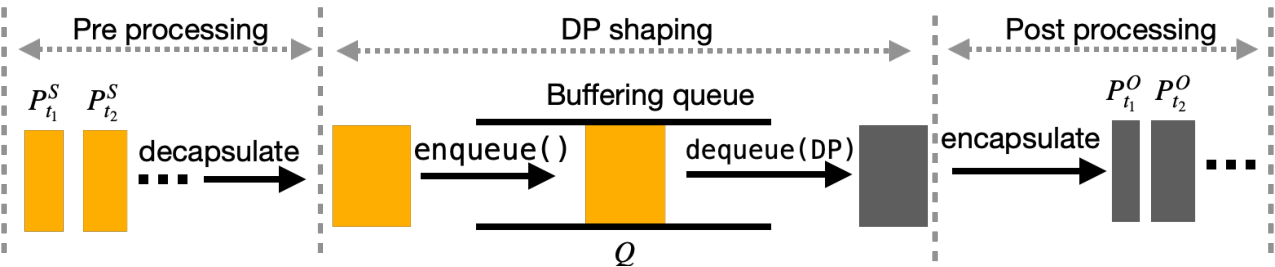
\includegraphics[width=\columnwidth]{figures/DPshaping_concept_vertical.pdf}
    %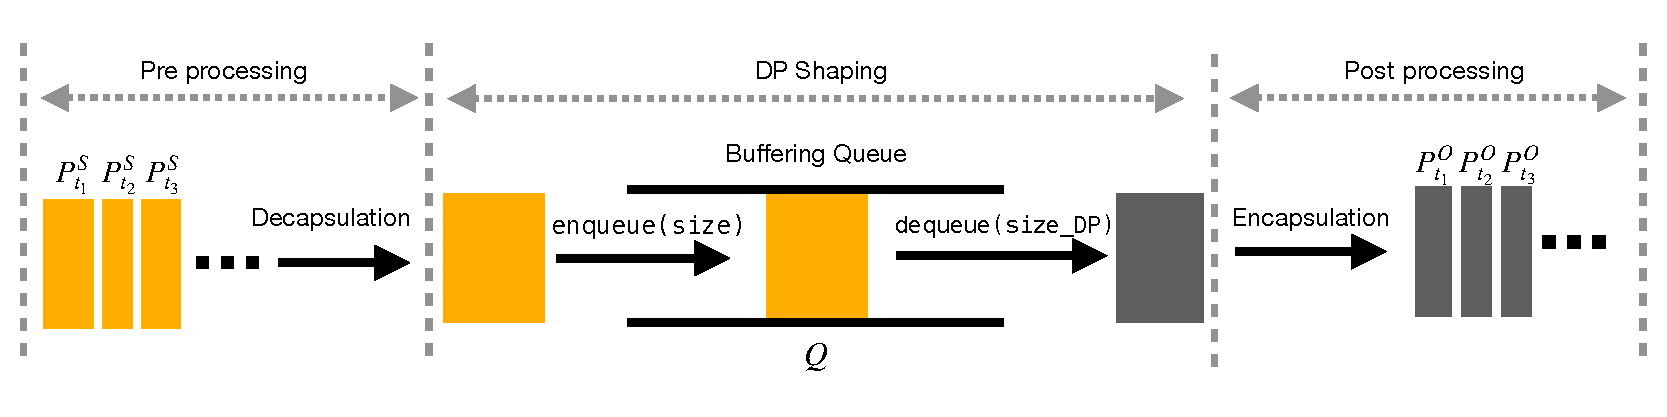
\includegraphics[width=\columnwidth]{figures/DPshaping_concept_horizontal.pdf}
    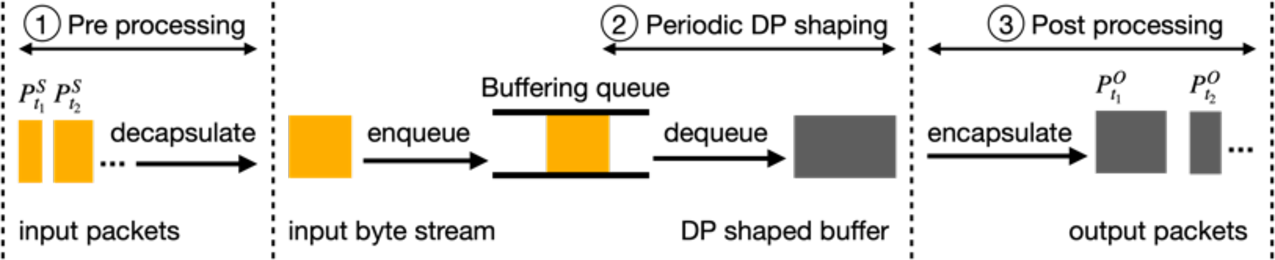
\includegraphics[width=\columnwidth]{dp-overview.pdf}
    \caption{Overview of DP shaping}
    \vspace{-0.4cm}
    \label{fig:dp-overview}
\end{figure}

The goal of differentially private shaping is to dynamically adjust packet
sizes and timing based on the available data stream, while ensuring that the DP
guarantees hold for any information that an adversary
(\S\ref{subsec:threat-model}) can observe.

%At a high level, \sys's DP shaping performs {\em DP measurements} of the amount
%of traffic to send, to adapt the shaped traffic size which preventing data
%leakage.
%
%To build the differentially-private shaping mechanism, we first define the
%``query'' on traffic streams that is subject to the DP mechanism. We call it a
%{\em DP measurement}, which measures the amount of application traffic available
%within a finite interval, adds noise to this amount according to the mechanism,
%and subsequently transmits a number of bytes equal to the noised amount.
%The DP shaping involves three steps (\Cref{fig:dp-overview}).
%First, the preprocessing step transforms an input stream $S$ over a window
%$\window$ into a byte stream, which is
%accumulated in a {\em buffering queue} $\unshapedQ$. (We denote the length of
%$\unshapedQ$ by $\qlen$.) Specifically, as application packets arrive, {\sys}
%extracts the payload bytes and enqueues them into $\unshapedQ$.
%\paragraph{Preliminaries.}
%\label{subsec:dp-preliminaries}
We first formally model an application's input stream as a packet sequence
$\istream = \{{P^{\istream}_1}, {P^{\istream}_2}, {P^{\istream}_3}, \dots \}$,
%{\as{why do we need a superscript here? it is already defined as $S$.}}
where ${P_i}^\istream = (l^{\istream}_i, t^{\istream}_i)$ indicates that the
$i$\textsuperscript{th} input packet in $\istream$ has length $l^{\istream}_i$
bytes and is transmitted at timestamp $t^{\istream}_i$.
We call the total duration of a finite stream $\streamduration^S
\triangleq \max t^{\istream}_i - t^{\istream}_1$.
%    \max t^{\istream}_i$.
%\am{We may need to address the boundaries of a single stream a bit more
%carefully. When a client starts streaming a video, what do we consider as the
%start time for the client-to-server stream? Is it the time of the first packet
%of the first segment request sent on the network or is it the time when the
%client ``clicked'' on a video to request it? Similarly, what do we consider as
%the start time for the server-to-client stream? Is it the time of the last
%packet of the segment request that generated the server response?}
%\ml{I don't know if we do need to address it all, but at least this is not the
%right place imh. Here we're talking about abstract streams, then one can decide
%to say "streams are when the button is clicked, and I compute if they're
%neighbors this way". Or am I missing something?}
Without shaping, an adversary can precisely observe $\istream$ and infer
the content, which is correlated with the~stream (\S\ref{subsec:attack-bg}).

%We assume that the finest granularities of packet sizes and timing that an
%adversary can observe are 1 byte and 1 ns, respectively.
%Thus, if $\istream$ has two consecutive packets as $(l_i, t_i)$ and $(l_j, t_j)$
%with $t_j = t_i + x$, then the adversary's effective observation between the two
%packets is $\{\cdots, l_i, 0_{(i+1)}, 0_{(i+2)}, \cdots, 0_{(i+x-1)}, l_j,
%0_{(i+x+1)}, \cdots\}$.
%We introduce this time granularity for clarity of explanation. We choose 1 ns as
%a reasonable time step that lets us observe individual packets in measurements,
%but a finer granularity can be swapped in without changing the guarantees.
%
%\update{
%For shaping, we define the primitive of a {\em buffering queue} $\buffQ$ to
%control the maximum amount of information subject to the DP mechanism and,
%hence, the sensitivity of the DP mechanism.
%}
%Conceptually, {\sys} extracts bytes from the input stream, $\istream$, and
%enqueues them in the buffering queue $\buffQ$.
%We denote the number of bytes present in $\buffQ$ (\ie length of the queue) by
%$\qlen$.

%\update{
%Additionally, we define a periodic interval, called a {\em DP measurement
%interval}, of length $\dpintvl$, which determines the frequency of applying the
%DP mechanism on traffic streams.
%For a DP measurement interval $[t_d,~t_d + \dpintvl)$ and a
%sub-sequence $\istream_d \subseteq \istream$ of the input stream that falls
%within the interval, \ie $\{P^{\istream}_i, \cdots P^{\istream}_j\}$ with
%$t^{\istream}_i \geq t_d$ and $t^{\istream}_j < t_d + \dpintvl$, the total
%application bytes accumulated in $\buffQ$ within the interval $\qlent{d} =
%\sum_{p=i}^{j} l^{\istream}_p$.
%}

\Cref{fig:dp-overview} provides a high-level overview of the
differentially-private shaping mechanism. Shaping happens in periodic intervals
of fixed length $\dpintvl$, called the {\em DP shaping intervals}.
\circled{1} As the packets in an application's stream arrive, the payload bytes
extracted from the packets are placed into a {\em buffering queue}, $\buffQ$.
\circled{2} In each periodic interval, the DP shaping algorithm
performs a {\em DP query}: it measures the length of $\buffQ$ with DP,
to determine the number of bytes to transmit in the next interval.
{\sys} then prepares a DP shaped buffer using the
payload bytes from $\buffQ$, and additional dummy bytes if required.
This shaped buffer is enqueued to be sent over the network at the end of
the DP shaping interval, right before the next interval starts.
\circled{3} Finally, data in the shaped buffer may be split into one or more
packets, as part of a post-processing step, and transmitted to the network.

The size of each shaped buffer generated in an interval has ($\varepsilon_{T},
\delta_{T}$)-DP guarantees. The per-interval guarantees
compose over a sequence of multiple intervals, thus providing DP guarantees for
traffic streams of arbitrary lengths. The guarantees degrade as the stream length increases (\Cref{prop:dp})

%We next elaborate on how this design enables \sys's formal DP guarantees.
%
We now discuss the steps of building a DP mechanism for
traffic streams in \S\ref{subsec:building-blocks} and the
%We show the complete differentially-private shaping workflow and discuss the
privacy guarantees in \S\ref{subsec:dp-queue-measurements}.
%Finally, we prove our guarantees in \S\ref{subsec:dp-proof}.

% \subsection{The Building Blocks}
% \label{subsec:infromation-bottleneck}

% \Cref{fig:dp-overview} illustrates {\sys}'s $(\epsilon,\delta)$-DP
% shaping strategy.
% %We denote an application's input packet sequence by
% An application's input stream is a packet sequence
% $\istream = {P^S_2}, {P^S_3}, \dots \}$,
% %{\as{why do we need a superscript here? it is already defined as $S$.}}
% where ${P_i}^S = (l^S_i, t^S_i)$ indicates that the $i$\textsuperscript{th} input
% packet in $S$ has length $l_i$ bytes and is transmitted at timestamp $t_i$.
% Without shaping, an adversary can precisely observe $\istream$ and infer
% the content,
% % which is any content that is correlated with this stream.
% which is correlated with the~stream~\cite{schuster2017beautyburst}.

%\paragraph{Goal.}
%The design of our traffic shaping algorithm relies on three key steps.
%The rest of this section is organized as follows.
%In \S\ref{subsec:infromation-bottleneck}, we formalize the information available
%to an attacker observing an application stream, which is the sequence of sizes,
%inter-packet intervals, and directions of packets at the finest granularity of
%observation.
%%We propose a primitive of a {\em buffering queue} to collapse all this
%%information into a sufficient statistic to adapt {\sys}'s transmission rate:
%%the
%%size of data in the queue waiting to be transmitted through our shaping
%%mechanism.
%%
%In \S\ref{subsec:dp-queue-measurements}, we describe our decision mechanism for
%sending data based on DP decisions.
%%We show how to perform {\em DP querys} of our buffering queue, in
%%order to adapt \sys's transmission rate with DP guarantees.
%%We show that under natural constraints on the transmission rate decision
%%mechanism, the change of queue size is bounded, allowing us to perform DP
%%measurements.
%%(\Cref{alg:dp_shaping_mechanism}).
%%Intuitively, we can use DP queue measurements and public information such as
%%network conditions to decide the amount of data to transmit.
%%Transmissions contain queued data when some is available, and dummy data
%%otherwise.
%%The stream observed by any attacker is a post-processing of the DP queries
%%issued on the queue (depends on the private data only through the DP
%%measurements), and is hence DP.
%%
%Finally, in \S\ref{subsec:dp-proof}, we provide a proof sketch for the DP
%guarantees of our shaping mechanism.

%{\as{I don't think we should summarize the intro of DP section into only one
%paragraph. We should give a summary of section here, explaining why we think DP
%shaping is a good idea and how it works Intuitively. More importantly, I think
%we need to  }}
%Specifically, given an application with a corpus of objects, the DP shaping
%ensures that each pair~of {\em neighbouring} objects---whose sizes are within a
%bounded distance---is indistinguishable under DP notion from the observations of
%their traffic shape.
%We denote the maximum distance between any pair of application objects by
%$\ssens$.
%
%Intuitively, {$\sys$} aims to ensure that a stream $S$ is indistinguishable (in
%the DP sense) from a neighboring stream $S'$ by observing the shaped traffic.

\subsection{DP for Traffic Streams}
\label{subsec:building-blocks}
% \subsection{The Sensitivity for DP Measurements}
% \label{subsec:sensitivity}

We now discuss the three steps for building a DP mechanism on
traffic streams. Specifically, we present our neighboring definition for
streams, define the DP query on streams that {\sys} runs and bounds its sensitivity,
and show the DP mechanism that we use to make the query DP.

%%%Defining neighboring streams on these sequences is challenging, since the
%%%lengths of different application streams as well as the packet sequences may
%%%have large variance, hiding which may require large amounts of noise. To bound
%%%this variance, we first transform an application's traffic stream into a {\em
%%%burst sequence}, i.e., a sequence of bursts transmitted in fixed-length
%%%intervals $\dpintvl$. Formally, we represent a burst sequence as: $\ibstream =
%%%\{{B^S_1}, {B^S_2}, {B^S_3}, \dots \}$, where ${B_i}^S = (L^S_i, i.\dpintvl)$
%%%indicates that the $i$\textsuperscript{th} burst in $S$ has length $L^S_i$
%%%bytes and is transmitted in the interval $i.\dpintvl$.

%The main primitive in \sys's DP adaptive shaping is a DP query of the
%buffering queue ($\buffQ$) size.
%As discussed in \S\ref{subsec:DP-background}, making a measurement DP requires
%three steps: defining a granularity of protection through a neighboring
%definition, bounding the sensitivity of the computation, and adding noise to the
%computation result.
%We describe the key ideas in \sys's design that make this possible.

\textbf{Step 1: Neighboring Definition.}
Building a DP mechanism requires a suitable definition of neighboring
streams, which requires a notion of distance between streams.
%Two streams are neighbors if their distance is below a configured threshold.
The neighboring definition has two implications. First, it
determines the sensitivity for a ``query'' subject to the DP mechanism and, in
turn, the amount of noise necessary for ensuring a given DP guarantee. Second,
it defines the granularity of privacy guarantee: intuitively, neighboring streams
are indistinguishable based on only the results of the DP mechanism applied to
them.
%\am{Is this about hiding between n and n+1 streams?}
%\ml{On really/only. It is n n+1 if your def covers the 0 stream. It is always
%about indistinguishability between two streams the are neighbors (ie you can't
%know if one or the other is running with high confidence---there's a discussion
%on that later for the DP semantics, towards the end. hopefully it makes it clear
%and we can remain high level here.)}
Hence, we aim for a neighboring definition for which ``streams have many
neighbors'', and the sensitivity of the DP query we want to run is as low as
possible.
%\am{We already discuss the two implications in the DP background in \S2.4. Is
%there a way to shorten this paragraph?}
%\ml{I think it's the first time we instantiate it for streams, so it seemed
%important to me. But I guess we can compact/delete if it's obvious and we
%need space?}
%\ml{should we use DP query instead of DP measurement?}

%\todo{
%Defining a distance over streams of arbitrary lengths would yield a weak
%neighboring definition, as differences accumulate over time.
%and all streams would be far from each other.
\update{Defining neighbors over streams has two challenges. First, the streams
can be arbitrarily long and the distance between streams would typically
increase with stream length. Secondly, if we consider streams with packet
timestamps at the finest granularity, the distance between the streams may be as
large as the sum of sizes of all packets in both streams. Both these factors
imply that a stream would either have few neighbors (enabling weak privacy), or
the neighboring definition would need to specify a large distance threshold,
requiring a lot of noise for strong DP guarantees.}
%\todo{Defining neighbors over streams of arbitrary lengths would be challenging,
%as the distance between streams would typically increase over time. As a result,
%a stream would either have few neighbors (weak privacy), or the neighboring
%definition would need to be based on a large distance threshold, requiring a lot
%of noise for strong DP guarantees.}
%}
% large values for sensitivity, which implies that shaping would require adding
% large amounts of noise to retain privacy.

To keep the neighboring distance threshold small, we take two steps.
First, we define the notion of a {\em neighboring window}, which is a time
interval of configurable length $\winlen$ over input streams.
For notational convenience, we set $\winlen$ as an integral multiple of the DP
shaping interval $\dpintvl$ and write
$\winlen = k \dpintvl$, although this is not a strict requirement.

%\ml{\sout{
%A finite sub-sequence $\istreamw \subseteq \istream$ that falls within the
%neighboring window is the packet sequence $\{P^{\istream}_i, \cdots
%P^{\istream}_j\}$ where $t^{\istream}_i \geq t_w$ and $t^{\istream}_j < t_w +
%\winlen$.
%}}
\update{Secondly, to measure the distance between streams over a neighboring
window, we consider the total bytes in each stream (burst lengths) transmitted
within coarse-grained time intervals and use the difference in the burst lengths
in the intervals within the window. Intuitively, we need an interval granularity
that is coarse enough to generate similar burst length sequences in more
streams, but is also small enough to bound the accumulation of differences over
time (to bound sensitivity, our next step).}
%\todo{
%We now need a notion of distance between two streams $\istream$ and
%$\istream'$ over a neighboring window $[t_w,~t_w +\winlen)$. To this end, we
%need to measure differences at a relevant granularity. Intuitively, we need a
%granularity that is coarse enough that differences between streams can average
%out, but small enough that we can later bound the accumulation of such
%differences over time (to bound sensitivity, our next step).
%%\am{I think the intuition for why we need the coarse granularity in the first
%place is not clear.}
%}
As will become clear with \Cref{prop:sensitivity}, the DP shaping
interval $\dpintvl$ is the coarsest granularity that we can use.
Hence, considering a neighboring window starting at a timestamp $t_w$, \ie
$[t_w,~t_w + \winlen)$,
we define the following representation of stream $\istream$ over the window
%Hence, we define the following representation of stream $\istream$ over a window
$[t_w,~t_w +\winlen)$ at granularity $\dpintvl$: $S_{t_w, W} = \{L^S_{t_w},
L^S_{t_w+\dpintvl}, L^S_{t_w+2\dpintvl}, \ldots, L^S_{t_w+(k-1)\dpintvl}\}$,
where $L^S_{t} \triangleq \sum_{(l^S_i, t^S_i) \in S} \1\{t^S_i \in [t,
t+\dpintvl)\} l^{\istream}_i$ is the total application bytes accumulated in
$\buffQ$ in the interval $[t, t+\dpintvl)$.

We now present the following neighboring definition:
\begin{definition}
\label{def:neighboring-streams}
Two streams $S$ and $S'$ are neighbors if, for any neighboring window
$[t_w,~t_w +\winlen)$, the L1-norm distance between their representations
$S_{t_w, W}$ and  $S'_{t_w, W}$  is less than $\ssens$.
Formally, $S$ and $S'$ are neighbors if:
\begin{equation}
\max_{t_w} {\norm{S_{t_w, W} - S'_{t_w, W}}}_1 \leq \ssens .
\end{equation}
\end{definition}
We utilize the L1-norm (the sum of absolute values) to quantify the distance
between two traffic streams, as it captures differences in both traffic size and
temporal alignment, at the granularity of $\dpintvl$.
%\ml{\sout{$\ssens$ is the maximum distance between neighboring streams and is
%computed as the max L1-norm of the difference between a pair of
%application
%streams in traffic bytes, over any neighboring window of length up to
%$\winlen$.}}
%
%
We will show (in \Cref{prop:sensitivity}) that despite our restriction
%\am{of defining neighboring streams over windows of at most length $\winlen$}
of defining neighboring streams at a granularity of $\dpintvl$, and of computing
distances over windows of length $\winlen$, we can quantify {\sys}'s DP
guarantees for streams at any granularity and of any length.
%\ml{maybe forward point to Prop 1, which doesn this?}

The neighboring window length $\winlen$ and neighboring distance
$\ssens$ are both configuration parameters, which are set before the start of an
application's transmission.
%\ml{
%%[[Note: moved.] I would move this entire discussion to the "Impact of DP
%%Shaping on Performance" header below. For now it is sufficient to know that
%%it's parameters and the order of magnitude I think. Later we can exlain how we
%%set it based on domain knowledge, and why, since we'll be ready to discuss
%%impact on perf.]
%In practice, setting $\winlen$ larger than $\streamduration_{max}$, the total
%length of the longest stream to be protected would yield $\ssens$ larger than
%the max distance of any stream pairs and incur unnecessary overheads.
%%and we require $\winlen \leq \streamduration_{max}$.
%On the other hand, the upper bound for $\ssens$ is the NIC's line rate times
%window length $\winlen$. While the upper bound value would ensure that all
%streams that can possibly be sent are neighbors with each other, yielding a
%strong DP guarantee and making any stream indistinguishable, it would also incur
%high overheads.
%%(\S\ref{}).
%%\am{Which section should we reference here?}
%%\ml{I don't know... I thought we evaluated the impact of W on overheads, but if
%%not we shouldn't ref anything}
%\todo{While smaller $\winlen$ implies smaller $\ssens$ (which would yield lower
%overheads) $\winlen$ is lower-bounded by the DP shaping interval $\dpintvl$,
%as will be clear in the subsequent paragraphs.}
%Typically, one would set $\winlen$ based on application
%domain knowledge, such as the fact that videos often consist of a sequence of
%segments requested at fixed intervals (\eg 5s) or the maximum size of a web
%request.
%}
In practice, $\winlen$ would be in the order of milliseconds to seconds.
Subsequently, one would determine $\ssens$ based on the typical
difference of traffic between application streams over windows of length
$\winlen$.
The practical upper bound for $\ssens$ is the NIC's line rate times
window length $\winlen$, but smaller values based on domain knowledge are
often possible.

\if 0
\paragraph{From windows to intervals.}
%\am{Add rationale for moving from $\winlen$ to $\dpintvl$.}
{Based on \Cref{assumption:window} and \Cref{def:neighboring-streams},}
the window length $\winlen$ affects the maximum number of bytes that can be
accumulated in the buffering queue (thus, the maximum distance between stream
pairs), as well as the transmission delay for the payload bytes enqueued.
Specifically, large windows lead to high-latency bursty traffic.
\shepherd{To reduce latency and burstiness}
\as{comment 1.b: we should explain how does having two windows reduce the
burstiness and why we cannot make W as small as T},
{\sys} further splits the neighboring windows into smaller intervals of length
$\dpintvl$, called the {\em DP shaping intervals}, and performs a {\em DP
measurement} at the beginning of each interval.
%
%The privacy loss over any window is now defined by applying DP composition
%on the privacy loss of intervals spanning the window.
%\ml{This is accurate, but would make way more sense (to me at least) as an
%    explanation/analysis {\bf after} we formally state the neighboring def, not
%    with definitions.}
\todo{Note that this quantization of application traffic into intervals is
essential for modeling the DP mechanism and the privacy, latency, and
bandwidth overheads. However, the model does not make any assumption about the
alignment of the actual traffic stream with the DP intervals.}
%Although an adversary can observe traffic at the finest granularities of packet
%sizes (\ie 1 byte) and timing (1 ns), we need to quantize the traffic to be able
%to model a DP mechanism as well as the privacy, latency, and bandwidth
%overheads.
\fi
%\update{At a high level, we have $\streamduration \geq \winlen > \dpintvl$. We
%    elaborate on parts of this relation later in this section.
%}

%\ml{This should go with the measurement. I think we should call it DP
%measurement and DP measurement interval in the overview, and then define it
%properly only when we actually define the measurement}
%Finally, we define the ``query'' on traffic streams that is subject to the DP
%mechanism. We call it a {\em DP measurement}, which measures the amount of
%application traffic available within a DP interval and adds noise to this amount
%according to the mechanism, to compute the number of bytes that must be
%transmitted in the interval. \am{Here or next subsection?}
%and subsequently transmits a number of bytes equal to the noised amount.

\textbf{Step 2: DP query and sensitivity.}
In {\sys}, a DP query measures the buffering queue length $\qlen$ with DP at
intervals $\dpintvl$. This noisy measurement determines the number of bytes
that must be transmitted in the interval.
%provide privacy guarantees.
To make the measurement of $\qlen$ differentially private, we need to bound the
sensitivity $\qsens$ of the queue length variable $\qlen$.
This sensitivity $\qsens$ is the maximum difference in $\qlen$ that can be
caused by changing one application stream to neighboring one. Formally, consider
two alternative neighboring streams $\istream$ and $\istream'$ passing through
the queue.
Suppose that when transmitting $\istream$ (similarly $\istream'$), the
queue length at time $k$ is denoted by $\qlent{k}$ (respectively $\qlent{k}'$).
Then, assuming w.l.o.g. that $k \geq k'$:
%\am{What does this assumption mean? That the two streams have
%different durations? Also, do we account for misaligned streams here?}
\setlength{\abovedisplayskip}{0pt}
\begin{equation}
    \qsens = \max_{k = 0}^{\streamduration}~\max_{\istream,
        \istream'} | \qlent{k} - \qlent{k}' |
    \label{eqn:ssens}
\end{equation}

Bounding $\qsens$ is still challenging though, as our neighboring definition
only bounds the difference in traffic between two streams over any window of
length upto $\winlen$.
Because of this, when $\streamduration >> \winlen$, differences between what
$\istream$ and $\istream'$ would enqueue in $\buffQ$ can accumulate over time,
and the difference betwen $\qlent{t}$ and $\qlent{t}'$ can grow unbounded over
time.
%\am{I don't fully understand the previous sentence. What does the neighboring
%streams definition and $\ssens$ have to do with the challenge of bounding
%$\qsens$.}\ml{is the above clearer now?}
% For long streams with $\streamduration >> \winlen$, differences between
% $\istream$ and $\istream'$ can accumulate and grow unbounded.

To bound $\qsens$, {\sys} relies on the key assumption that
the tunnel can always transmit all incoming data from
application streams within any $\winlen$-sized time window. That is,
%\ml{Is it the tunnel, or just the buffering queue?}
%\am{I think only the buffering queue needs to be able to flush the bytes, but t
    %is okay to be a little vague here.}
%In other words, we assume that:
%is that the tunnel can handle all incoming data from application streams within
%$\winlen$-sized window of time.
%Specifically, we make the following assumption:
\begin{assumption}\label{assumption:window}
All bytes enqueued prior to or at time $t$ are transmitted by time $t+W$.
\end{assumption}
%\ml{I'm making this more concrete as it's very useful for the discussion of W
%and T}
To enforce this assumption, {\sys} implements a time to live in the buffering
queue, flushing all bytes older than $\winlen$ from $\buffQ$ (see
\S\ref{sec:design} for more details).
%\ml{[Do we actually give these details? I didn't see it. Ideally we could add
%them, but if not let's just remove this sentence.]
%We give details about this tunnel design in \S\ref{sec:design}.}
%\am{In the eval section, we discuss values of $\winlen$ that simply satisfy our
%flushing requirement. Our system implementation and probably even design does
%not support it explicitly. I think we should say something in the design about
%tracking the expiry time of each byte in $\buffQ$ and then Shaper dropping
%expired bytes.}
%\ml{would make sense to me, but if we have space I guess?}
%\ml{Do we explain that somewhere? Should we actually explain it here (dropping
%the queues) so that we can discuss the $W$ and $T$ tradeoff in this section?}
%
Intuitively, this assumption caps the accumulation of traffic differences in
$\buffQ$ to the maximum difference over $\winlen$, \ie $\ssens$.
Since the size of $\buffQ$ cannot differ by more than $\ssens$ when changing a
stream by a neighboring one, the difference between DP query results of $\buffQ$
under two neighboring streams---which is the sensitivity of the DP query,
$\qsens$---is upper-bounded by $\ssens$. Formally:

\begin{proposition}\label{prop:sensitivity}
    {$\sys$} enforces $\qsens \leq \ssens$.
\end{proposition}

\begin{proofsketch}
Consider any two streams $\istream$ and $\istream'$, as in \Cref{eqn:ssens},
and any measurements time $k$.
The proof proceeds in two steps. First, under \Cref{assumption:window},
streams can accumulate queued traffic for at most {$\winlen$}, so two
different streams can create a difference $|\qlent{k} - \qlent{k}'|$ of at
most $\ssens$.
Second, dequeuing can only make two different queues closer: Consider
query time $k$, with queue lengths $\qlent{k} > \qlent{k}'$ (the
opposite case is symmetric).
For a DP noise draw $z$, we have $\qlendpt{k} > \qlendpt{k}'$. Since shaping
sends at least as much data under $\qlendpt{k}$ as under $\qlendpt{k}'$,
but no more than $\qlendpt{k} - \qlendpt{k}'$, after dequeuing we have
$|\qlent{k+1}' - \qlent{k+1}| \leq |\qlent{k}' - \qlent{k}|$.
In summary, the queue difference under two different streams
$\qsens$ can grow to at most $\ssens$ due to data queuing, and dequeuing only
decreases that difference, and hence $\qsens \leq \ssens$.  The complete
proof is in \S\ref{appendix:dp}.
\end{proofsketch}

% We can now reason about DP guarantees over intervals of length $\dpintvl$ in
% order to achieve the privacy loss for streams over longer transmission
% durations.
% We discuss this in \S\ref{subsec:dp-proof}.

%and we can bound the sensitivity of $\qsens \leq \ssens$.
%We defer the proof, which requires accounting for DP noise, to
%\S\ref{subsec:dp-proof}, Proposition~\ref{prop:sensitivity}.

%\ml{This shouldn't be here I think. We're talking about DP, and going from one
%measurement to many will be handled by composition in the next section. The
%discussion between $W$ and $T$ can happen at the end in the discussrion of the
%implications of our design for performance. I don't think it should be in the
%middle of this.}
%\am{Needs discussion?}

\if 0
\paragraph{Bounding Sensitivity.}
The second step in providing DP measurements is to bound the sensitivity of the
computation we want to make private. Remember that we aim to measure the state
of traffic to adapt the amount of shaped traffic we send.
Since the sensitivity is the worst case change in result between two neighboring
streams, we need to reason about the worst case change to any measurement we want
to make, when performing this measurement on two adjacent streams.
We defined adjacent streams in terms of the difference of amount of traffic sent
over time, but there could be large differences in packetization, making it
difficult to bound the impact on any measurement.
%
\sys's key idea is to use the primitive of a {\em buffering queue} to control
the maximum information accessible by a measurement, and hence the sensitivity
of the computation.
Conceptually, {\sys} extracts bytes from the input stream, $\istream$, and
enqueues them in the buffering queue $\buffQ$.
We denote the number of bytes present in $\buffQ$ (\ie length of the queue) by
$\qlen$.

With this primitive in place, we are now ready to define our DP measurement and
analyze its sensitivity. We use subscript $T$ to denote measurement specific
quantities.
As $\qlen$ is the amount of application data waiting in $\buffQ$ to be sent, we
would ideally want {\sys} to move $\qlen$ bytes from $\buffQ$ to the shaped
buffer, for it to be sent over the network.  Hence {\sys} measures $\qlen$, with
DP to provide privacy guarantees. To make the measurement DP we need to bound
$\qsens$, the sensitivity of $\qlen$, which is the maximum difference in the
queue length $\qlen$ that can be caused  by changing one application stream to
neighboring one.
Formally, consider two alternative neighboring streams $\istream$ and
$\istream'$ passing through the queue.
Suppose that when transmitting $\istream$ (similarly $\istream'$), the
queue length at time $t$ is denoted by $\qlent{t}$ (respectively $\qlent{t}'$).
Then, assuming without loss of generality that $\streamduration \geq
\streamduration'$:
\setlength{\abovedisplayskip}{0pt}
\begin{equation}
    \qsens = \max_{t = 0}^{\streamduration}~\max_{\istream,
        \istream'} | \qlent{t} - \qlent{t}' |
    \label{eqn:ssens}
\end{equation}

Bounding $\qsens$ is still challenging thought, as our neighboring definition
only bounds the difference in traffic between two streams over any window of
length $\winlen$.
For long streams with $\streamduration >> \winlen$, differences between
$\istream$ and $\istream'$ can accumulate and grow unbounded.
\fi

%To bound sensitivity, {\sys} relies on the key assumption that
%\todo{the tunnel can always transmit all incoming data from
%application streams within any $\winlen$-sized time window.}
%\ml{Is it the tunnel, or just the buffering queue?}
%In other words, we assume that:
%%is that the tunnel can handle all incoming data from application streams within
%%$\winlen$-sized window of time.
%%Specifically, we make the following assumption:
%\begin{assumption}\label{assumption:window}
%  All bytes enqueued \todo{prior to or} at time $t$ are transmitted by time
%  $t+W$.
%\end{assumption}
%We explain how to realize this assumption in a tunnel design in
%\S\ref{sec:design}.
%\ml{Do we explain that somewhere? Should we actually explain it here (dropping
%the queues) so that we can discuss the $W$ and $T$ tradeoff in this section?}
%%
%Intuitively, this assumption caps the accumulation of traffic differences in
%$\buffQ$ to the maximum difference over $\winlen$, and we can bound the
%sensitivity of $\qsens \leq \ssens$. We defer the proof, which requires
%accounting for DP noise, to \S\ref{subsec:dp-proof},
%Proposition~\ref{prop:sensitivity}.

\textbf{Step 3: Adding Noise.}
With sensitivity bounded at $\ssens$, we can now query $\qlen$ with DP using
an additive noise mechanism, which entails sampling noise $z$ from a DP
distribution and computing the DP buffer queue length as $\qlendpt{k} \triangleq
\qlent{k} + z$.
Specifically, {\sys} uses the Gaussian mechanism, in which
the noise $z$ is sampled from a centered normal distribution
$z \sim \mathcal{N}\big(\mu,~\sigma^2\big)$, where the variance is parameterized
by $\epsilon_\dpintvl$, $\delta_\dpintvl$, and~$\ssens$:
$\sigma^2 =
(2\ssens^2)/(\varepsilon_\dpintvl^2)\ln(1.25/\delta_\dpintvl)$.
%\frac{2\ssens^2}{\varepsilon_\dpintvl^2}\ln(\frac{1.25}{\delta_\dpintvl})$.
Parameters $\epsilon_\dpintvl$, $\delta_\dpintvl$ determine the amount of
noise added to each DP query~result.
%\ml{[Let's keep that for the proof.]\sout{Under this noise distribution, one
%measurement is \mbox{$(\epsilon_\dpintvl, \delta_\dpintvl)$-DP}.}}


\subsection{Privacy Analysis}
\label{subsec:dp-queue-measurements}

The previous section defines $(\varepsilon_{\dpintvl}, \delta_{\dpintvl})$-DP
guarantees for the traffic transmitted in an individual shaping interval. We now
discuss (i) the guarantees for longer
application streams, (ii) the guarantees on a packet-level sequence derived from
a shaped buffer sequence, and (iii) the privacy implications for streams that
fall outside of the neighboring definition.

\textbf{Guarantees for streams.}
Recall from the previous section that shaping happens at intervals
$\dpintvl$; in each interval we perform a DP query on the buffering queue length
$\qlen$ and create a shaped buffer of length $\qlendp$, which is subsequently
queued for transmitting over the network at the end of the interval.
%
%\ml{yeah maybe DP shaping interval is a better name for $\dpintvl$...}
Enqueueing data into the shaped buffer at the end of each shaping interval
creates a sequence of states for the shaped buffer $\{(\qlendp_1, T),
(\qlendp_2, 2T), (\qlendp_3, 3T), \dots \}$.
%\ml{can we get better notation for this?}
Although this sequence is not technically observable by an adversary, this is
where we prove our DP guarantees using DP composition over queries
performed during the stream transmission.
%while the stream is running (\S\ref{subsec:dp-proof}).

\begin{proposition}\label{prop:dp}
For any stream $\istream$ of duration $\streamduration^S \leq
\streamdurationcfg$, {$\sys$}
enforces $(\varepsilon, \delta)$-DP for the sequence $\{(\qlendp_1, T),
(\qlendp_2, 2T), (\qlendp_3, 3T), \dots \}$, with $\varepsilon, \delta
\triangleq \textrm{DP\_compose}(\varepsilon_T, \delta_T, \lceil
\frac{\streamdurationcfg}{\dpintvl} \rceil)$.
\end{proposition}

\begin{proof}
Consider two neighboring streams $\istream$ and $\istream'$. By design, the
times at which shaped buffers are queued are independent of application data, so
$\{(\qlendp'_1, T'), (\qlendp'_2, 2T'), (\qlendp'_3, 3T'), \dots \} =
\{(\qlendp_1, T), (\qlendp_2, 2T), (\qlendp_3, 3T), \dots \}$, and we can
restrict our considerations to the sequences $\{\qlendp_1, \qlendp_2, \qlendp_3,
\dots \}$ and $\{\qlendp'_1, \qlendp'_2, \qlendp'_3, \dots \}$.
By Prop. \ref{prop:sensitivity}, the sensitivity of each measurement is at most
 $\ssens$.
By the Gaussian DP mechanism, the measured queue size $\qlendp$ in each
interval is $(\varepsilon_{T}, \delta_{T})$-DP.
Using DP composition over the $\lceil \frac{\streamdurationcfg}{\dpintvl}
\rceil$ DP queries made during any duration $\streamdurationcfg$
%$(\varepsilon_{T}, \delta_{T})$-DP,
 yields the ($\varepsilon, \delta$)-DP guarantee.
\end{proof}
We use R\'enyi-DP composition on the Gaussian mechanism for
$\textrm{DP\_compose()}$. {\sys} provides a DP guarantee for streams of any
length $t$, with the guarantee degrading gracefully as DP composition (of
order $\sqrt{\streamdurationcfg}$ as the length grows).
%\am{broken sentence?}\ml{just forgot to close the parents}
%If $\winlen$ is larger than all traffic streams, {$\sys$} enforces
%$(\varepsilon_{\winlen}, \delta_{\winlen})$-DP over all streams going through he
%shaped tunnel. \am{Not sure what the previous statement is trying to
%say.}{\as{I also think maybe it is better to remove it}}

%\todo{Note that the overhead (\ie noise added) due to DP does not depend on the
%number of streams: the overhead is the same regardless of the number of streams
%transmitted through the buffering queue simultaneously.}
%\am{Organize it.}

\textbf{Guarantees for packet sequences.}
Data from the shaped buffer is sent over the network, and transmitted as a
packet sequence denoted by $\ostream = \{{P^O_1}, {P^O_2}, {P^O_3} \dots \}$.
These packets are a post-processing of the DP-shaped buffer. As long as the
packets are generated independently of any secret data, they preserve the
DP guarantees of shaping due to the post-processing property of DP.
This yields the following result, directly implied by \Cref{prop:dp}
and DP post-processing:
\begin{corollary}
\label{cor:dp}
For any stream $\istream$ of duration $\streamduration^S \leq
\streamdurationcfg$, {$\sys$}
enforces $(\varepsilon, \delta)$-DP for its output packet sequence
\ostream,
with $\varepsilon, \delta \triangleq \textrm{DP\_compose}(\varepsilon_T,
\delta_T, \lceil \frac{\streamdurationcfg}{\dpintvl} \rceil)$.
\end{corollary}

\textbf{Privacy for non-neighboring streams.}
%Finally, if two streams are not neighboring for the parameter $\ssens$, but with
Finally, if the distance between two streams is larger than $\ssens$, \eg say
$k\ssens$ for some factor $k$, {\sys} still provides a (degraded) DP guarantee
through group privacy \cite[Theorem 2.2]{dwork2014algorithmic} applied to the
Gaussian mechanism.
Namely, a DP query in each shaping interval $\dpintvl$ for the non-neighboring
stream provides $(k\epsilon_\dpintvl, \delta_\dpintvl)$-DP, and the guarantees
can be extended for the stream duration $\streamduration$ by applying DP
composition to this new value.


\textbf{Interpretation of the guarantees.}
\update{
%By buffering all data in a queue, and periodically deciding the size of
%the data to send over the network with a DP measurement,
\sys's shaping algorithm provides a ($\varepsilon_{\dpintvl},
\delta_{\dpintvl}$)-DP guarantee on the volume of application
traffic enqueued (in the buffering queue) in a fixed-length interval
(and, by post-processing, the volume of traffic observable on the network).
%The timing of shaped buffer enqueueing however is not protected by DP.
}
%This is why {\sys} enforces a constant timing for this queueing, at intervals
%of length $\dpintvl$.
%With such a constant timing, DP holds for all observable traffic, as shown in
%\Cref{prop:dp} and Corollary \ref{cor:dp}.
%\ml{is that the correct summary for timing?}
%\update{However, we note that this constant timing is enforced as a best effort
%due to our use of generic hardware, as detailed in \S\ref{}.}.
%
Under perfect timing for the DP shaping interval $\dpintvl$, the DP guarantee
ensures that two neighboring streams, \ie their contents, are indistinguishable
with the probability as defined in \Cref{eq:dp}. Smaller
$\varepsilon_{\dpintvl}$ and $\delta_{\dpintvl}$ implies higher noise in
shaping, which increases the uncertainty about the original stream in the shaped
traffic.
%(the lower $\epsilon$ and $\delta$, the higher the noise added and higher the
%uncertainty).
%Thus, an attacker cannot distinguish the content of stream from that of any
%neighboring stream.

%\update{Secondly, the DP guarantees are independent of the number of streams
%transmitted simultaneously through the buffering queue.}
%\am{\sout{Finally, if $\ssens$ is large enough for all streams to be neighbor
%with a stream that doesn't send any data, {\sys} also hides the presence of any
%one stream.
%%between the tunnel endpoints.
%Thus, an attacker cannot distinguish the number of streams with high
%precision, including whether zero or one streams are running.}}
%{Note that because the DP guarantees can be shared among all the streams
%multiplexed through the buffering queue simultaneously, the overhead (\ie
%noise added) due to DP gets amortized among the streams.}
%\ml{[Suggestion: Replace all above with from ``Secondly'' by:]
Secondly, to enforce the DP guarantees, the DP noise of the Gaussian
mechanism does not depend on the total number of flows. Intuitively, the DP
guarantee is shared among all the streams multiplexed through the buffering
queue simultaneously for a fixed amount of noise, and the overhead (\ie noise
added) gets amortized among the streams.
%}

%\begin{algorithm}
%\DontPrintSemicolon
%\caption{DP Shaping Mechanism
%    \am{Redundant}
%
%\KwIn{$Q_{DP}, Q_{dummy}$}
%\KwOut{$Q_{QUIC}$}
%
%\While{True}{
%%\texttt{sleep($T$)}\;
%%\texttt{enqueue($Q_{DP}, \{P_{t_1}^S, P_{t_2}^S, \dots\}$)}\;
%$\qlen$ = \texttt{len($Q_{DP}$)}\;
%$\qlendp$ =  \texttt{DP\_measurement($\qlen$)}\;
%$R$ = \texttt{$\min(\qlen, \qlendp)$}\;
%%$R$ = \texttt{dequeue($Q_{DP}, \min(\qlendp, \qlen)$)}\;
%$D$ = $\qlendp > R~?~\qlendp - R : 0$\;
%$outbuf$ = \texttt{dequeue($Q_{DP})$ + dequeue($Q_{dummy})$}\;
%\texttt{enqueue($Q_{QUIC}, outbuf$)}\;
%%$P_{t_1}^O, P_{t_2}^O, \dots $ = \texttt{QUIC\_send($Q_{QUIC}$)}
%}
%%\;
%\end{algorithm}

% \begin{figure}
%   \centering
%   \begin{minipage}{0.8\linewidth}
%     \begin{algorithm}H]
%       \caption{DP Shaping Mechanism}
%       \KwData{$P_{t_1}^S, P_{t_2}^S, \dots $}
%       \KwResult{$P_{t_1}^O, P_{t_2}^O, \dots $}

%       \While{True}{
%         \texttt{sleep($T$)}\;
%         \texttt{enqueue($Q_{DP}, \{P_{t_1}^S, P_{t_2}^S, \dots\}$)}\;
%         $\qlendp$ =  \texttt{DP\_measurement($Q_{DP}$)}\;
%         $R$ = \texttt{dequeue($Q_{DP}, \min(\qlendp, \qlen)$)}\;
%         $D$ = $\qlendp - R$\;
%         \texttt{enqueue($Q_{QUIC}, R + D$)}\;
%         $P_{t_1}^O, P_{t_2}^O, \dots $ = \texttt{QUIC\_send($Q_{QUIC}$)}}\;
%     \end{algorithm}
%   \end{minipage}
%   \caption{Description of the DP Shaping Mechanism}
% \end{figure}

\begin{figure}[t]
    \centering
    %  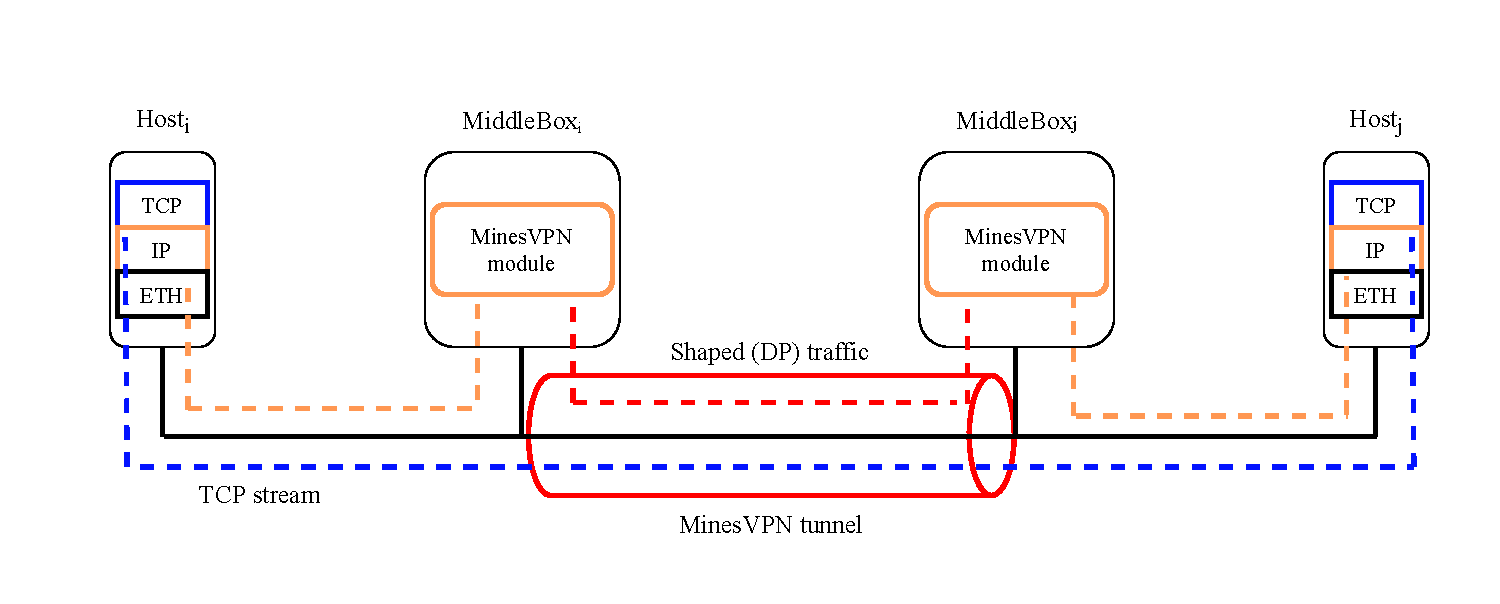
\includegraphics[width=\columnwidth]{figures/Design_highlevel.pdf}
    %  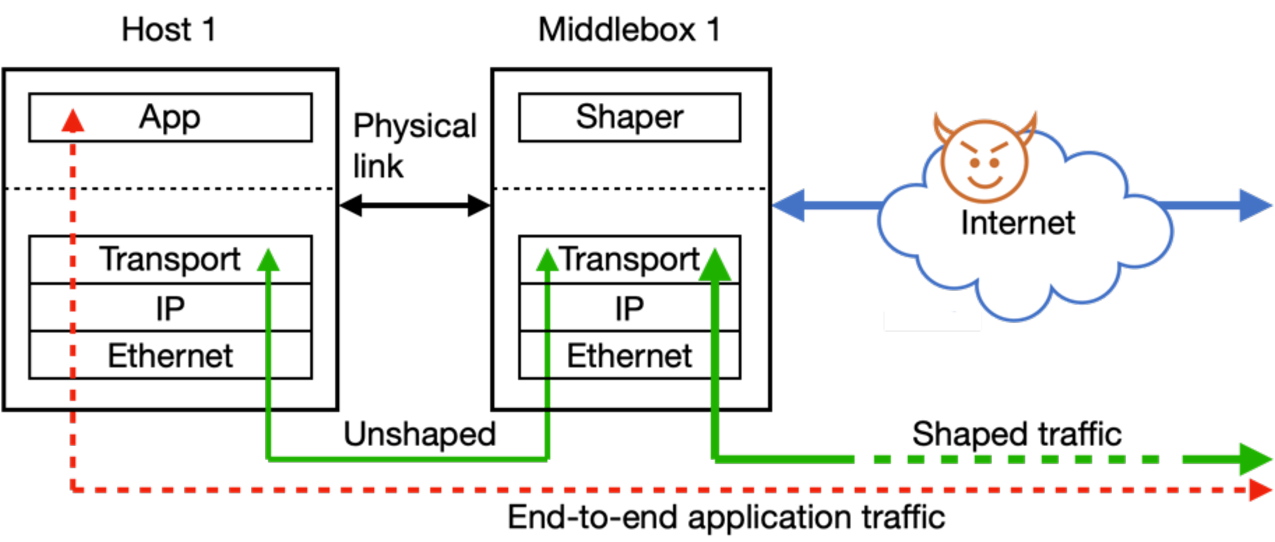
\includegraphics[width=\columnwidth]{figures/minesvpn-overview-half.pdf}
    %  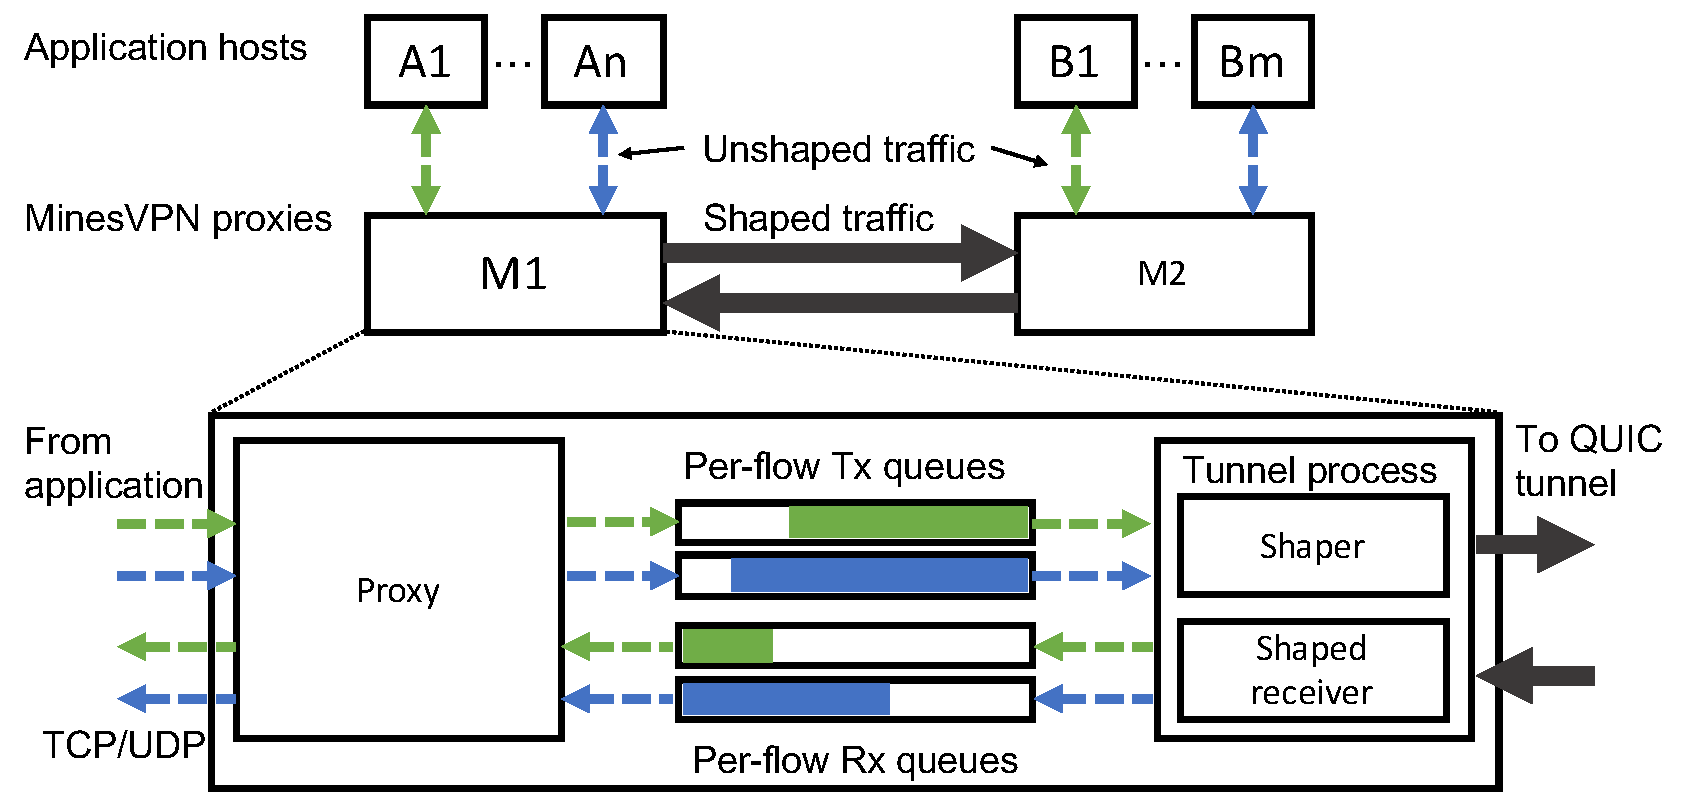
\includegraphics[width=\columnwidth]{figures/minesvpn-arch4.pdf}
    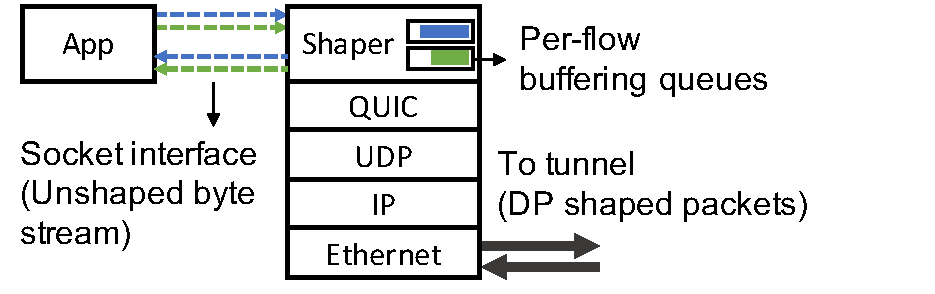
\includegraphics[width=\columnwidth]{design2.pdf}
    \caption{Overview of tunnel design (one endpoint)
        %\am{Update figure}
    }
    \vspace{-0.4cm}
    \label{fig:minesvpn-overview}
\end{figure}




\textbf{Privacy vs Performance.}
\sys's shaping mechanism introduces several parameters which impact privacy and
performance, specifically latency and bandwidth overheads. These parameters
include $\varepsilon_\dpintvl$, $\delta_\dpintvl$, $\ssens$, $\winlen$, and
$\dpintvl$.
%
%DP parameters $\ssens$, and ($\varepsilon_\dpintvl,
%\delta_\dpintvl)$ trade-off stronger privacy guarantees
%%(larger $\ssens$ strengthens the neighboring definition, and
%%$(\epsilon_\dpintvl, \delta_\dpintvl)$ the DP guarantee)
%for noisier measurements.
Larger $\ssens$ requires lower $\varepsilon_{\dpintvl}$ for stronger privacy,
which implies noisier measurements.
Noisy measurements imply more overhead---when the noise is positive, dummy bytes
need to be sent, incurring higher bandwidth overhead; when the noise is
negative, fewer bytes are sent and the unsent bytes accumulated in the buffering
queue incur a latency overhead.
This is the privacy-overhead trade-off we expect from DP.

Additionally, the parameters $\dpintvl$ and $\winlen$ have a more subtle impact
on the privacy-overhead trade-off.
%effect that also impacts the privacy-performance trade-off.
Traffic is shaped in intervals of $\dpintvl$; thus, $\dpintvl$ impacts the
latency and burstiness of the traffic.
A smaller $\dpintvl$ provides lower transmission latency and smaller bursts per
interval. However, it also requires more DP queries and, thus, incurs higher
privacy loss when transmitting the complete stream of a given length
$\streamduration$.
In practice, one would set $\dpintvl$ to the maximum value that can minimize
privacy loss while providing tolerable latency.

%$\winlen$ has a symmetric effect on privacy: a larger $\winlen$ for a fixed
%\todo{A practical upper bound for $\winlen$ is $\streamduration_{max}$, the
%total length of the longest stream in the neighboring set to be protected;
%$\winlen > \streamduration_{max}$ would yield $\ssens$ larger
%than the max distance of any stream pairs and incur unnecessary overheads.
%}
%On the other hand,
A large $\winlen$ for a fixed $\ssens$ implies that
neighboring streams can differ by at most $\ssens$ over a longer window size
$\winlen$, which weakens the neighboring definition and, hence, the privacy
guarantees.
%One would thus be tempted to make $\winlen$ as small as possible, maybe as small
%as $\dpintvl$.
While smaller $\winlen$ is desirable, the lower bound is $\dpintvl$.
Recall that, to bound $\qsens$ (\Cref{assumption:window}),
{\sys} must drop any bytes left in the buffering queue for longer than $\winlen$.
%older than $\winlen$ from the buffering queue.
Since data leaves the buffering queue in each shaping interval after a
DP query, setting $\winlen = \dpintvl$ would lead to immediate dropping of the
bytes from the buffering queue that aren't transmitted in response to the
DP query. This would happen \update{in each interval where the DP query samples
a negative noise value}.
%\am{for the first time?}\ml{no I mean "every time" here, is there a better way
%to say it?}.
These data drops would degrade {\sys}'s performance in terms of both
throughput and latency. Hence, we need $\winlen >> \dpintvl$ to ensure that data
has time to leave the buffering queue before it is too old.
Typically, one would set $\winlen$ based on application domain knowledge, such
as the maximum size of a web request or the fact that videos often consist of a
sequence of segments requested at 5s intervals.

We analyze the impact of different choices for these parameters on
the privacy guarantees and overheads in \S\ref{sec:eval}.

%\ml{Let's make sure this discussion addresses this at least:}
%\shepherd{To reduce latency and burstiness}\as{comment 1.b: we should explain
%how does having two windows recduce the burstiness and why we cannot make W as
%small as T}


\if 0

Specifically, large windows lead to high-latency bursty traffic.
\shepherd{To reduce latency and burstiness}\as{comment 1.b: we should explain how does having two windows recduce the burstiness and why we cannot make W as small as T}

\ml{[TODO: with at least this info taken from other places while moving things]
%
, {\sys} further splits windows into
smaller intervals of length $\dpintvl$ and samples noise at the beginning of
each interval.
\todo{Note that this quantization of application traffic into intervals is
essential for modeling the DP mechanism and the privacy, latency, and
bandwidth overheads. However, the model does not make any assumption about the
alignment of the actual traffic stream with the DP intervals.}
%\todo{In absence of shaping, the queue length corresponds to the amount of
%    unshaped traffic transmitted in an interval of $\dpintvl$.}
The privacy loss over a window is now defined by applying DP composition
on the privacy loss of individual intervals.
\am{Should the text from the beginning of this paragraph until the previous
sentence appear earlier as a justification for why we have separate $\winlen$
and $\dpintvl$?}
%
The privacy loss ($\varepsilon_{\winlen}$) and bandwidth overheads of the DP
shaping (represented by $\sigma_\dpintvl$, \ie the standard deviation of the
noise distribution function) depend on
$\winlen$, $\ssens$,
%$\varepsilon_{\dpintvl}$, $\delta_{\dpintvl}$,
and the number of intervals $\varnumupdates = \numupdates$ in $\winlen$.
Additionally, the latency overheads depend on $\dpintvl$.
Note that for a specific value of $\ssens$ and $\varnumupdates$, the DP guarantee
$\varepsilon_{\winlen}$ is fully specified by $\sigma_\dpintvl$, and remains the same even at
different time scales.
That is, scaling $\winlen$ and $\dpintvl$ proportionally does not change the
privacy and overhead costs.
%{\as{We are not sure about this, the latency can be affected by the amount of
%noise in extreme scenarios}}
}
\ml{[moved from above when I suggested removing]
In practice, setting $\winlen$ larger than $\streamduration_{max}$, the total
length of the longest stream to be protected would yield $\ssens$ larger than
the max distance of any stream pairs and incur unnecessary overheads.
%and we require $\winlen \leq \streamduration_{max}$.
On the other hand, the upper bound for $\ssens$ is the NIC's line rate times
window length $\winlen$. While the upper bound value would ensure that all
streams that can possibly be sent are neighbors with each other, yielding a
strong DP guarantee and making any stream indistinguishable, it would also incur
high overheads (\S\ref{}).
\am{Which section should we reference here?}
\ml{I don't know... I thought we evaluated the impact of W on overheads, but if
not we shouldn't ref anything}
\todo{While smaller $\winlen$ implies smaller $\ssens$ (which would yield lower
overheads) $\winlen$ is lower-bounded by the DP shaping interval $\dpintvl$,
as will be clear in the subsequent paragraphs.}
Typically, one would set $\winlen$ based on application
domain knowledge, such as the fact that videos often consist of a sequence of
segments requested at fixed intervals (\eg 5s) or the maximum size of a web
request.
}

\fi



\if 0
\subsection{Privacy Guarantees}
\label{subsec:dp-proof}
{\sys} provides ($\varepsilon_{\dpintvl}, \delta_{\dpintvl}$)-DP guarantees for
each DP measurement interval. Using this guarantee, one can then reason about DP
guarantees over a sequence of multiple intervals using DP composition methods.
In particular, for a transmission duration of length $D$, which consists of
$\lceil \frac{D}{\dpintvl} \rceil$ DP shaping intervals, {\sys} would provide
($\varepsilon_{D}, \delta_{D}$)-DP, with $\varepsilon_{D}, \delta_{D} \triangleq
DP\_compose(\varepsilon_{\dpintvl}, \delta_{\dpintvl}, \lceil \frac{D}{\dpintvl}
\rceil)$. We use R\'enyi-DP composition on the Gaussian mechanism for
$\textrm{DP\_compose()}$.
\am{Does this require proof?}

\if 0
%\as{I think we need to change the title of this section as it is not the proof
%but also proposing our guarantees. I suggest the title: "Privacy guarantees".}
At a high level, analyzing the  ($\varepsilon_{\winlen}, \delta_{\winlen}$)-DP
guarantee of the overall shaping mechanism requires two steps: (i) showing that
the difference in the buffering queue length is bounded for neighboring streams
for all transmissions of the streams (Prop. \ref{prop:sensitivity}), and (ii)
composing the DP cost of each measurement over the intervals defining a window
of length $\winlen$ (Prop. \ref{prop:dp}).
%\todo{(i) two neighboring streams in windows of length $\winlen$ are neighbors
%during all transmit intervals of length $\dpintvl$, and (ii) the total privacy
%loss composed over all transmit intervals within a window amounts to the privacy
%loss defined over the entire window.}
%\am{Verify wording.}
%\as{I think the wording is wrong for both points. We need to show that
%difference in queue lengths are bounded. Then the second point naturally follows
%by composition.}
%(i) the neighboring definition over the buffering queue length over intervals
%$\dpintvl$ implies neighboring definition

%Formally, {$\sys$} offers the following guarantee:
We first show that the sensitivity of each measurement $\qsens$ is at most the
window sensitivity $\ssens$:
\begin{proposition}\label{prop:sensitivity}
    {$\sys$} enforces $\qsens \leq \ssens$.
\end{proposition}

\begin{proofsketch}
  Consider any two streams $S_j$ and $S_j'$, as in \Cref{eqn:ssens}.
  The proof proceeds in two steps. First, under \Cref{assumption:window},
  streams can accumulate queued traffic for at most {$\winlen$}, so two
  different streams can create a difference $|\qlent{k} - \qlent{k}'|$ of at
  most $\ssens$.
  Second, dequeuing can only make two different queues closer: Consider
  measurement time $k$, with queue lengths $\qlent{k} > \qlent{k}'$ (the
  opposite case is symmetric).
  For a DP noise draw $z$, we have $\qlendpt{k} > \qlendpt{k}'$. Since shaping
  sends at least as much data under $\qlendpt{k}$ as under $\qlendpt{k}'$,
  but no more than $\qlendpt{k} - \qlendpt{k}'$, after dequeuing we have
  $|\qlent{k+1}' - \qlent{k+1}| \leq |\qlent{k}' - \qlent{k}|$.
  In summary, the maximum queue difference under two different streams
  $\qsens$ can grow to at most $\ssens$ due to data queuing, and dequeuing only
  decreases that difference, and hence $\qsens \leq \ssens$.  The complete proof
  is in \S\ref{appendix:dp}.
\end{proofsketch}

We can then reason about DP guarantees over intervals of length $\dpintvl$ in
order to achieve the privacy loss for the entire window of length $\winlen$.
%
\ml{[TODO Mathias] make notation consistent: here we want only the stream length
and then use W as a numerical application. This will show that we can compose over time}
Formally, we have:
\begin{proposition}\label{prop:dp}
  {$\sys$} enforces $(\varepsilon_{\winlen}, \delta_{\winlen})$-DP, with
  $\varepsilon_{\winlen}, \delta_{\winlen} \triangleq
  \textrm{DP\_compose}(\varepsilon_T, \delta_T, \numupdates)$.
\end{proposition}

\begin{proof}
By Prop. \ref{prop:sensitivity}, the sensitivity of each measurement is at most
  $\ssens$.
%\am{I thought the sensitivity is already defined in \Cref{eqn:ssens}.}
By the Gaussian DP mechanism, the measured queue size $\qlendpt{k}$ in each
interval $k$ of length $\dpintvl$ is $(\varepsilon_{T}, \delta_{T})$-DP.
% Over a time window of length $\winlen$, {\sys} will sample noise
% $\numupdates$ times.
Using DP composition over $\numupdates$ $(\varepsilon_{T}, \delta_{T})$-DP
measurements, and the fact that $\ostream$ is a post-processing of DP
measurements, yields the ($\varepsilon_{\winlen}, \delta_{\winlen}$)-DP over
any $\winlen$ length window.
% By using R\'enyi algorithm for DP\_compose(), we get $\varepsilon$,
% $\delta$ that correspond to ($\varepsilon_{\winlen}, \delta_{\winlen}$)-DP
% definition over $\winlen$ windows.
%\todo{Thus, the proof concludes with the application of DP composition.}
%\am{I am not sure how the last line follows from the second last line: what does
%it mean say proof concludes with application of DP composition.}
%\as{It is just the way of saying that compositions is applied here and privacy
%parameters, $\varepsilon_W, \delta_W$ are result of it.}
\end{proof}
We use R\'enyi-DP composition on the Gaussian mechanism for
$\textrm{DP\_compose()}$.
%If $\winlen$ is larger than all traffic streams, {$\sys$} enforces
%$(\varepsilon_{\winlen}, \delta_{\winlen})$-DP over all streams going through he
%shaped tunnel. \am{Not sure what the previous statement is trying to
%say.}{\as{I also think maybe it is better to remove it}}
Note that the overhead (\ie noise added) due to
DP does not depend on the number of streams: the overhead is the same regardless
of the number of streams transmitted through the buffering queue simultaneously.
\fi


%\smallskip\noindent
\paragraph{Summary.}
By buffering all data in a queue, and periodically deciding the size of the data
to send over the network with a DP measurement, \sys's shaping algorithm
makes the shape of traffic (volume of data sent over time) DP with regards to
the application's original traffic sequence.
%The DP shaping algorithm ensures that an adversary cannot trace the observed
%packet sizes on the network back to the packet sizes in the application's
%original sequence.
% The DP shaping algorithm makes \ml{the amount of traffic \sout{the packet sizes}
% output} on the network independent of (DP with regards to) the amount of traffic
% in the application's original sequence, in each window of size $\winlen$.
% of the packet sizes in the application's
% original sequence.
% \ml{[this is wrong without the later timing things I think, shoule remove? Or at
% least should be refined, I'm not too sure what the goal is here] Furthermore,
% due to the periodic execution of algorithm and the subsequent DP post processing
% property, the timing of output packets is also independent of the packet timings
% in the original sequence.}
Thus, as long as no observable characteristics of the traffic directly depend on
application secrets (the original traffic sequence), the observable outbound traffic
is DP.
% Thus, the algorithm ensures that the shape of the outbound traffic of an
% application is independent of application secrets.

%\am{The proof of the DP guarantees of the algorithm is provided in the
%appendix. Can we prove that constant timing intervals + differentially privacy
%on size = differentially privacy on the overall traffic shape?}

\ml{\paragraph{Interpretation} Let's add something on interpreting the guarantees and what they mean here: hidding any marginal change of size sensitivity (presence + content); composition over time; group composition for larger sensitivity.}
\ml{[This is from the intro]
\am{Clarify that our shaping will provide DP on transmission sizes only. For
timing we rely on fixed intervals.}
%
The adversary can observe sizes, inter-packet intervals, and directions of
packets in sequences of arbitrary lengths.
Given these observations, the specific DP guarantee that {\sys} provides is that
the adversary cannot identify (i) the traffic content (\eg video streams, web
pages), and (ii) the presence of any one flow between two application
endpoints.
}
\ml{
{\sys}'s DP guarantees \todo{cover} all (overlapping) windows up to size
$\winlen$, and composes over larger windows.
}
\ml{Here we want to discuss group composition and the neighboring definition in general}

\fi

%%%%%%%%%%%
%% old text
%%%%%%%%%%%
% \paragraph{Unshaped queue.}
% We model an abstract queue, {$\unshapedQ$}, which holds the unshaped input byte
% stream of an application and supports two operations: enqueue and dequeue.

% \paragraph{Neighboring queue states.}
% We define the queue state, ${\unshapedQ}_{\tau}$, as the amount of traffic
% inside ${\unshapedQ}$ at time $\tau$. We call two queue states, ${\unshapedQ}_{\tau}$
% and ${\unshapedQ}'_{\tau}$, neighbor queue states if and only if we have:
% \begin{equation}\label{equ:queue-neighboring}
        % |{\unshapedQ}_{\tau} - {\unshapedQ}'_{\tau}| \leq D_q \;(bytes)
% \end{equation}
% where $D_q$ is a parameter in our system.


% \paragraph{Query function and sensitivity.}
% We define a query function on the queue state ${\unshapedQ}$,
% $f({\unshapedQ}_{\tau})$, as a function that returns the
% size of the queue at time ${\tau}$. The sensitivity of the function $f$ is given~by:
% \begin{equation}
% \Delta_1 f = \max_{Q, Q'} \| f(Q_{\tau}) - f(Q'_{\tau}) \|_1 =  \max_{Q, Q'} \| Q - Q' \|_1 = D_q
% \end{equation}
% Here, $\Delta_1 f$ captures the magnitude by which the size of queue can change
% from one stream to another.  In fact, {\sys}'s shaping strategy guarantees that
% the queue size cannot be accurately ascertained by an attacker.  At this point,
% we have all necessary building blocks to propose our differentially private
% shaping algorithm.

% \paragraph{From queues to traffic streams.}

% The definition presented in \Cref{equ:queue-neighboring} serves as a sufficient
% basis for designing our differentially private traffic shaping based on queue
% states.  However, in order to provide comprehensive privacy guarantees for
% internet applications, we extend this definition from queue states to
% streams of traffic.


% To reason about the privacy of traffic streams, we need to define neighboring
% streams (i.e. the minimal protection unit of each differentially private
% algorithm).  Two stream prefixes, $S_t$ and $S'_t$ (with the representation of
% \Cref{equ:stream-segs}), are neighbors if and only if:
% \begin{equation}\label{equ:stream-neighboring}
        % \|S_t - S'_t\|_1 \leq D_s \; (bytes)
% \end{equation}
% We utilize the L1-norm as our distance metric to quantify the dissimilarity
% between two traffic streams, as it captures differences in both
% segment size and temporal pattern.


% Our goal is to measure, and subsequently bound, the privacy loss of a traffic
% stream.
% Intuitively, an attacker's observation of a traffic stream can be interpreted as
% a series of differentially private queries on the segment sizes of original
% traffic pattern. \am{I find this intuition of an attacker issuing DP queries
% strange. To me, the attacker performs usual queries on a database whose
% underlying distribution has been made DP.}
% We claim that the privacy loss for a individual traffic stream shaped with our
% mechanism can be quantified by aggregating the privacy loss incurred at each
% measurement of the abstract queue size.
% The following statement provides a formal representation of this notion.


% \ml{Amir, please use real latex things for the Claim and Lemma. I'd also call the Lemma Proposition instead: Lemma is for general theoretical tools others might reuse and apply to other proofs).}
% \textbf{Claim}: The privacy loss of transmitting a traffic stream with the
% length of $w = kT$ through the {\sys} middle-box, is the composition of $k$
% queries on the queue state.
% \\
% To show that this claim is true, we only need to prove the following lemma.

% \textbf{Lemma}: Assume two neighboring traffic streams, $S_t$ and $S_t'$,
% transmitted through a middle-box with \Cref{alg:middle-box-all} as the shaping
% mechanism. If they both reshaped to the same traffic stream, $S_O$, then,  at
% any given time $\tau$, the queue states for neighboring streams are $D$-close.
% In other words we have:
% \begin{equation}\label{equ:composition_dp_section}
        % \forall \tau > 0 : |Q_{\tau} - Q_{\tau}'| \leq D
% \end{equation}
% where $D = \min(D_q, Q_{max})$. $D_q$ and $Q_{max}$ are the queue neighboring
% threshold and maximum buffer size of our middle box respectively.
% \am{I see no relation between $D_q$ and $D_s$.}

% This means the unshaped queues of these two streams are always neighbors
% according to the neighboring definition of \Cref{equ:queue-neighboring}.
% We prove the Lemma in \Cref{appendix:dp}.

% Here, we show how we can calculate privacy loss for a traffic stream.
% Assume two neighbor streams, $S_t$ and $S_t'$, reshaped to the same stream,
% $S_O$, by {\sys} middle-box. If we show the shaping mechanism by $M_s$, the
% privacy loss is:
% \begin{equation}\label{equ:privacy-loss}
  % \log\big(\frac{\Pr[M_s(S_t)=S_O]}{\Pr[M_s(S_t')=S_O]}\big) \leq \varepsilon_g
% \end{equation}
% Using the representation of \Cref{equ:stream-segs}, we have:

% \todo{Add the equation}

% The composition comes into the picture in the inequality \todo{Add ref} as the
% size of output at each round depends on the amount traffic enqueued into the
% ${\unshapedQ}$ and outputs of previous rounds of the mechanism, which both
% abstracted in the queue state.

\if 0
\subsection{DP shaping building blocks}
\label{subsec:infromation-bottleneck}
We define a source application stream $S$ as a sequence of packets
$\{P_{t_1}^{l_1}, P_{t_2}^{l_2}, P_{t_3}^{l_3}, \dots \}^S$
%$\{P_{t_1}^{l_1}, P_{t_2}^{l_2}, P_{t_3}^{l_3}, \dots \}^S = \langle(l_1, t_1),
%(l_2, t_2), (l_3, t_3), \dots \rangle^S$,
where $l_i$ and $t_i$ respectively indicate the length in bytes and timestamp of
the $i$\textsuperscript{th} packet of the stream $S$.
%\begin{equation}\label{equ:stream-pkts}
%        $S = \{P_{t_1}^S, P_{t_2}^S, P_{t_3}^S, \dots \}$,
%\end{equation}
%where $P_{t_i}^S$ is the size of the packet transmitted as a part of the stream
%$S$ at the time $t_i$.
%
Without shaping, an adversary can observe this precise stream and infer
the content, which is correlated with this stream.

In {\sys}, we first introduce an information bottleneck in the form of a
buffering queue, {$\unshapedQ$}, to control the information accessible by an
eavesdropper. The buffering queue has three operations: \texttt{enqueue(size)},
\texttt{dequeue(size)}, \texttt{get\_size()}.
Conceptually, {\sys} decapsulates all application traffic of incoming stream
$S$, and enqueues it in the {$\unshapedQ$}.
The shaping mechanism in {\sys} periodically retrieves the queue size and
determines the amount of data to dequeue from $\unshapedQ$ in order to transmit
it as shaped traffic.
The shaped traffic is encapsulated into a new sequence of packets, which we
denote as:
\begin{equation}\label{equ:stream-segs}
    O = \{P_{t_1}^O, P_{t_2}^O, P_{t_3}^O, \dots\}
\end{equation}
where $P_{t_i}^O$ is a packet sent in the shaped tunnel.

In order to ensure that the observable stream $O$ preserves the privacy of the
original stream $S$, {\sys} ensures that $O$ is Differentially Private.
To enforce DP, {\sys} ensures that any input to $O$ that depends on sensitive
data (the stream $S$) is measured with DP.
\Cref{fig:dp-overview} shows the end-to-end traffic shaping of {\sys}.
After decapsulating incoming packets, the incoming traffic is stored in a
buffering queue. In fixed periods, the \texttt{dequeue} operation is performed,
ensuring that the timing of the outgoing traffic remains independent of the
incoming traffic. The size of the \texttt{dequeue} is determined by our
differential privacy mechanism, guaranteeing that the size of the outgoing
traffic remains DP.
Furthermore, the encapsulation and packetization of outgoing data can be
characterized as a post-processing step of a differentially private mechanism
and therefore is DP.
\fi


\if 0
\subsection{DP shaping mechanism}
\label{subsec:dp-shaping}

\ml{I feel like this all belong to \am{design} with the DP call as a noisy black
box.} \am{Yes, this is covered in \S\ref{subsec:design-overview}.}

\Cref{alg:middle-box-all} represents the differentially private shaping
mechanism.  The algorithm is executed periodically with an interval of $T$
seconds.  Here, we explain one round of the algorithm.
\begin{enumerate}
  \item The DP mechanism reads the current size of the queue, $Q_t$.
  \item Then, it adds a noise from a Gaussian distribution with an average of
  zero and scale of ${\sigma}$ to the current size. The noisy measurement is
  represented by $D^S_t$ in the algorithm, and $\sigma$ is the parameter that
  determines the privacy loss of our mechanism.
  \item To avoid unpredictable behaviors such as the occurrence of negative
  values in the noisy measurement, we have incorporated a minimum and maximum
  size threshold for the noisy measurements, which are adjustable parameters
  within the algorithm.
  \item If $D^S_t > Q_t$, the data in {\unshapedQ} will be padded to $D^S_t$
  bytes and subsequently transmitted to the receiver.
  Conversely, if the size of the data in {\unshapedQ} is less than or equal to
  $D^S_t$, the entirety of the $D^S_t$ bytes will be sent.  In algorithm
  \ref{alg:middle-box-all}, the padding size and real data size are represented
  with $D^P_t$ and $D^R_t$ respectively.
\end{enumerate}
\fi


\if 0
\noindent
\am{Outline:\%\%\%\%\%\%\%\%}
\begin{itemize}
    \item \S 3.1: DP background
    \begin{itemize}
        \item ($\varepsilon, \delta$)-DP definition
        \item Components for building a DP mechanism: neighboring definition,
        query on the dataset and the sensitivity for that query given the
        neighboring definition, noise mechanism
        \item DP properties relevant for {\sys}: post processing, composition,
        robustness to auxiliary knowledge
    \end{itemize}
    \item \S 3.2: Building blocks for a DP mechanism on traffic streams
    \begin{itemize}
        \item Neighboring definition: define window $W$, assumption 1,
        definition 1
        \item Query on streams: call this DP query here, define buffering
        queue abstraction, DP interval $T$, explain why $T < W$.
        \item Define the noising mechanism: the additive gaussian noise
        mechanism from shaping overview
    \end{itemize}
    \item \S 3.3: Workflow of {\sys}'s DP shaping and privacy guarantees
    \begin{itemize}
        \item DP workflow: shaping overview (move notations to 3.2)
        \item DP guarantees: ($\varepsilon_W, \delta_W$)-DP through a
        composition of a series of ($\varepsilon_T, \delta_T$)-DP querys.
        \item How we use DP properties: post processing, composition, and
        robustness to aux. knowledge?
    \end{itemize}
    \item \S 3.4: Proof sketch: Mostly fine, may only require notational
    clarification.
\end{itemize}
\am{End of Outline:\%\%\%\%\%\%\%\%}
\fi


